\chapter{成果展示}
  \label{chap:成果展示}
    本次的项目基本完成了商城前端部分的开发,功能演示如下。
    \section{商城模块}
      \label{sec:商城模块}
        商城页效果如图(\ref{fig:home_my}),
        \begin{figure}[htbp]
          \centering
          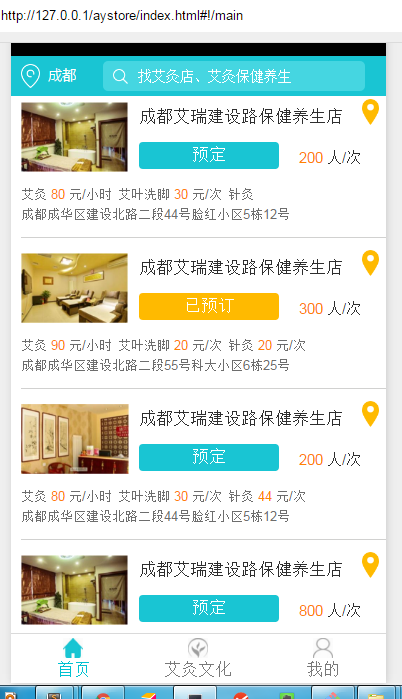
\includegraphics[width=5cm]{./img/home_my.png}
          \caption{商城页的效果展现}
          \label{fig:home_my}
        \end{figure}
        % \begin{figure}[htbp]
        %   \centering
        %   \subfigure[1]{
        %   \begin{minipage}{5cm}
        %     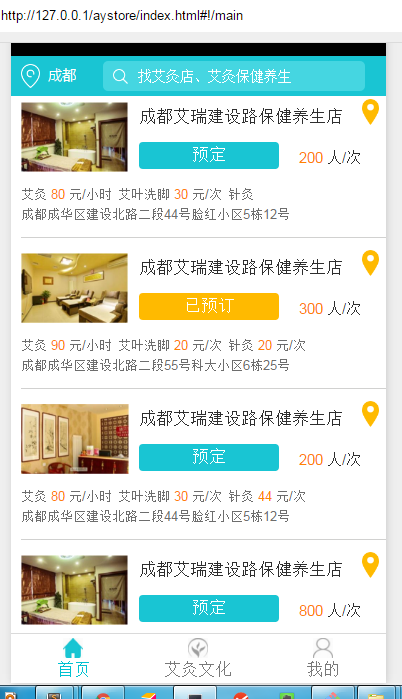
\includegraphics[width=5cm]{./img/home_my.png}
        %     \caption{商城页的效果展现}
        %     \label{fig:home_my}
        %   \end{minipage}
        %   }%
        %   \subfigure[1]{
        %   \begin{minipage}{5cm}
        %     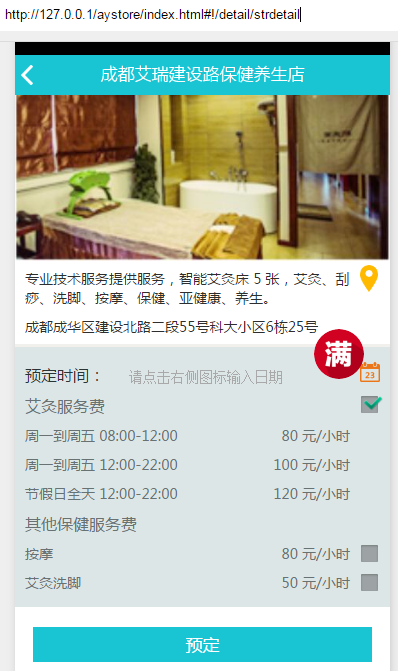
\includegraphics[width=5cm]{./img/strdetail_my.png}
        %     \caption{店铺详情的效果展现}
        %     \label{fig:strdetail_my}
        %   \end{minipage}
        %   }
        % \end{figure}
        这个页面上的数据不是静态的,而是通过 http 请求特定格式的 json 数据后填充的;店铺详情的效果如图(\ref{fig:strdetail_my}),
        \begin{figure}[htbp]
          \centering
          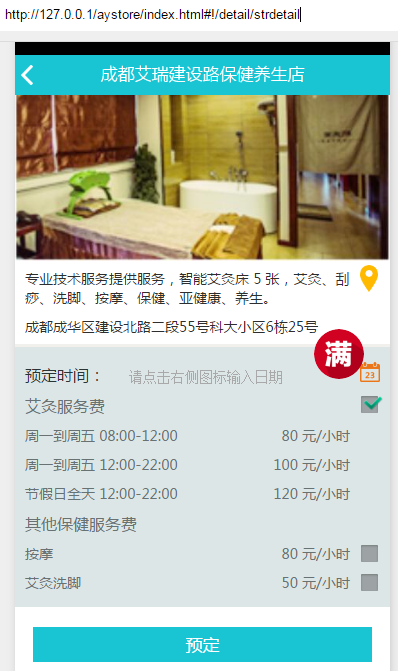
\includegraphics[width=5cm]{./img/strdetail_my.png}
          \caption{店铺详情的效果展现}
          \label{fig:strdetail_my}
        \end{figure}
        复选框的样式和设计图存在出入,设计图见(\ref{fig:strdetail_my}),但不影响基本功能,可以选择日期和时间,可以选择其他的服务。点击预定后进入下一页,可以继续选择人数等;支付页如图(\ref{fig:pay_my}),
        \begin{figure}[htbp]
          \centering
          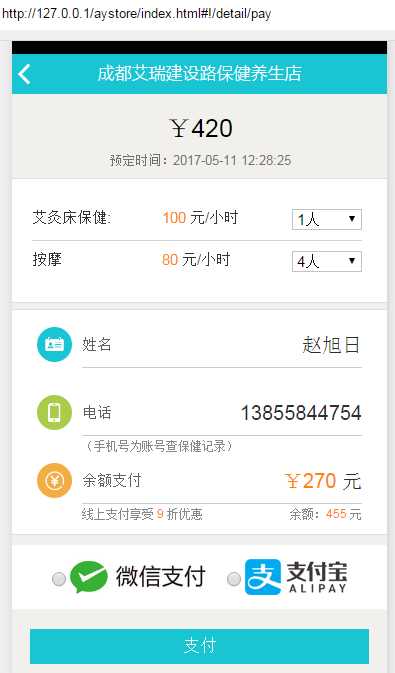
\includegraphics[width=5cm]{./img/pay_my.png}
          \caption{支付页的设计效果展现}
          \label{fig:pay_my}
        \end{figure}
        当选择人数时,上面可以实时现实总价;支付成功页如图(\ref{fig:pay_successful_my}),
        \begin{figure}[htbp]
          \centering
          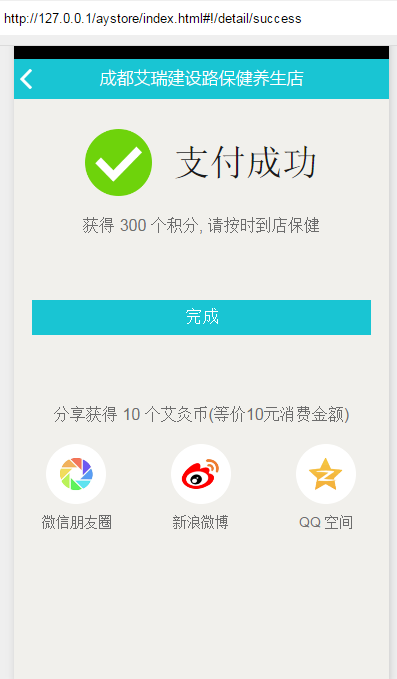
\includegraphics[width=5cm]{./img/pay_successful_my.png}
          \caption{支付成功页的设计效果展现}
          \label{fig:pay_successful_my}
        \end{figure}
        与设计图基本相符。

    \clearpage
    \section{文章模块}
      \label{sec:文章模块}
        文章列表页的效果如图(\ref{fig:artlist_my}),
        \begin{figure}[htbp]
          \centering
          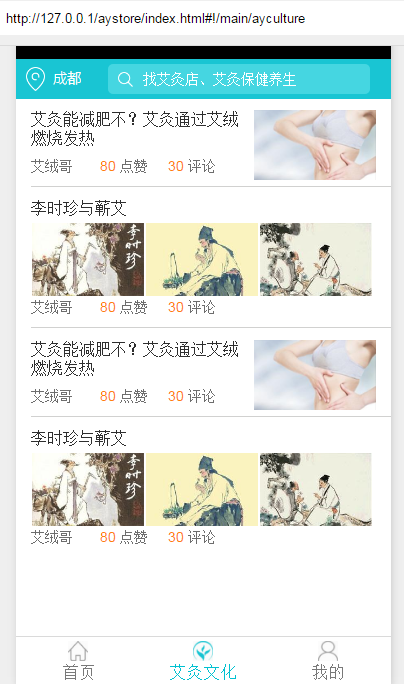
\includegraphics[width=5cm]{./img/artlist_my.png}
          \caption{文章列表页的效果展现}
          \label{fig:artlist_my}
        \end{figure}
        基本的信息都可以展示,这些数据也是通过 http 服务请求特定的数据而加载的,点击文章的任意一条后,跳转到文章详情页,如图(\ref{fig:artdetail_my}),
        \begin{figure}[htbp]
          \centering
          
\includegraphics[width=5cm]{./img/artdetail_my.png}
          \caption{文章详情页的效果展现}
          \label{fig:artdetail_my}
        \end{figure}
        点击收藏图标或喜欢图标后,图标会黄色,提示已经收藏或点赞,再次点击按钮又变为灰色。

    \clearpage
    \section{我的空间模块}
      \label{sec:我的空间模块}
        我的页效果如图(\ref{fig:mine_my}),
        \begin{figure}[htbp]
          \centering
          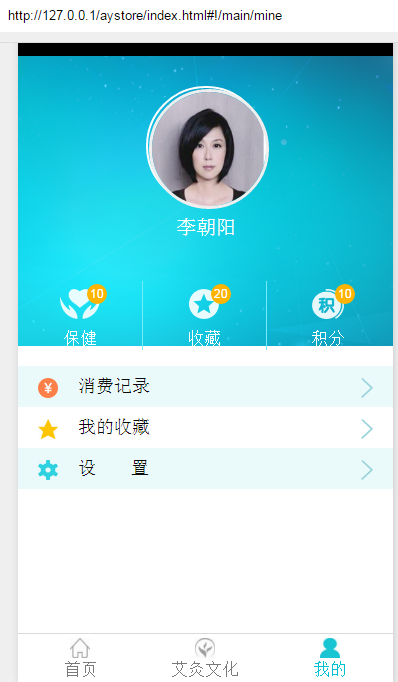
\includegraphics[width=5cm]{./img/mine_my.png}
          \caption{我的页效果展现}
          \label{fig:mine_my}
        \end{figure}
        点击消费记录一栏会进入消费记录页,如图(\ref{fig:record_my}),
        \begin{figure}[htbp]
          \centering
          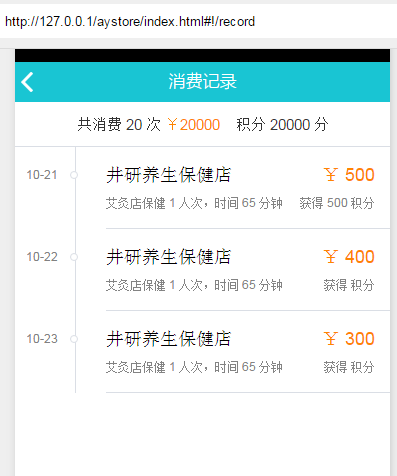
\includegraphics[width=5cm]{./img/record_my.png}
          \caption{消费记录页的效果展现}
          \label{fig:record_my}
        \end{figure}
        返回后,点击设置一栏会进入设置页,如图(\ref{fig:setting_my})。
        \begin{figure}[htbp]
          \centering
          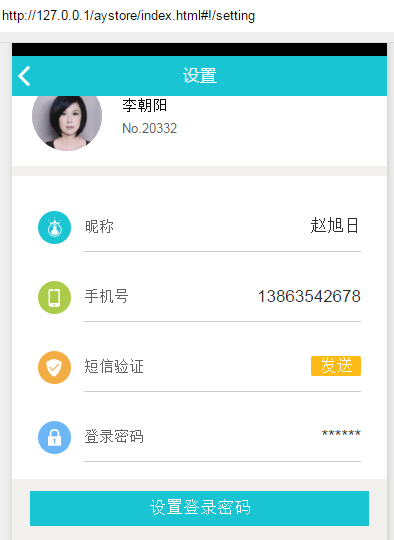
\includegraphics[width=5cm]{./img/setting_my.png}
          \caption{设置页效果展现}
          \label{fig:setting_my}
        \end{figure}

    \clearpage
    \section{本章小结}
      \label{sec:效果总结}
        以上我的项目目前所能实现的效果,不过还有很多功能未能实现,与理想的目标还有很长距离。
